\documentclass[runningheads]{llncs}
\usepackage[T1]{fontenc}
\usepackage[utf8]{inputenc}
\usepackage{graphicx}
\usepackage{booktabs}
\usepackage{amsmath,amssymb}
\usepackage{url}
\usepackage{color}
\renewcommand\UrlFont{\color{blue}\rmfamily}
\setlength{\textfloatsep}{7pt plus 2pt minus 2pt}
\setlength{\floatsep}{7pt plus 2pt minus 2pt}

\begin{document}
\title{From Observation to Action: When Does Hypothesis Testing Help Agents Discover Hidden Rules?}
\titlerunning{Hypothesis Testing for Hidden-Rule Discovery}
\author{Arti}
\authorrunning{Arti}
\institute{IILM University, Greater Noida, India}
\maketitle

\begin{abstract}
Agents in new environments must infer hidden rules from the consequences of their actions. We ask when explicit hypothesis testing helps, comparing a hypothesis-driven agent with reactive, posterior-sampling and learned agents in two synthetic environment families: a procedural grid world with six generalization regimes and a combination vault. At moderate difficulty, agents given testable macro-actions perform similarly, but differences emerge at harder levels where structured evidence tracking and information-seeking become important. A key question is whether the advantage of hypothesis testing comes from its decision mechanism or from its explicit representation of uncertainty. In the main matched-information comparison, a learned Macro-GRU supplied with the hypothesis tracker's structured beliefs matches the hypothesis agent at the hardest difficulty, while an ordinary Macro-GRU without belief features trails substantially. A 30-seed rule-permutation re-evaluation on unseen colors reproduces this pattern: the hypothesis tracker and Macro-GRU+belief both achieve 0.980, compared with 0.611 for Macro-GRU and 0.554 for Macro-FF; posterior sampling reaches 0.862. The hypothesis-transfer variant reaches 1.000. These results indicate that the principal advantage in this benchmark comes from structured access to uncertainty over hidden rules rather than from the hypothesis-testing policy mechanism itself. Evidence is from synthetic, deterministic environments with hand-built skill vocabularies; we make no claim about ARC-AGI-3 or general intelligence.
\keywords{Rule discovery \and Hypothesis testing \and Posterior sampling \and Compositional generalization \and Learned agents.}
\end{abstract}

\section{Introduction}
Agents deployed in new environments rarely get the rules explained; they must infer them from the consequences of their own actions: which key opens which door, which lever order unlocks a vault. This is close in spirit to measuring skill-acquisition efficiency rather than skill on a fixed distribution~\cite{chollet2019}. Three mechanisms are commonly proposed: explicit \emph{hypothesis testing}~\cite{klahr1988,gopnik1997,tenenbaum2011}, Bayesian \emph{posterior sampling}~\cite{strens2000,osband2013}, and \emph{learned} policies whose recurrent state implements adaptation~\cite{duan2016,wang2016}. We compare them in controlled, fully inspectable benchmarks and ask four questions. \textbf{Q1:} does explicit hypothesis testing beat reactive, Bayesian and learned agents, and where? \textbf{Q2:} which ingredients (reward form, information bonus, memory, revision, structural assumptions) account for the differences? \textbf{Q3:} must the testable-action vocabulary be supplied, or can a learned agent find it from generic skills? \textbf{Q4:} do the findings replicate in a second, structurally different environment family?

This is an independent benchmark study; it does not reproduce ARC-AGI-3 or any external benchmark, uses no language models, and makes no claim about general intelligence. \textbf{Contributions.} (1) A procedural grid-world benchmark with six generalization regimes and rule-type and assumption-violation variants, plus a second family (a combination vault). (2) A hypothesis-driven agent, a posterior-sampling agent, and learned agents over testable macro-actions, over generic skills and over primitives, with three training seeds for the learned agents. (3) A factorial ablation separating reward form from the information bonus. (4) A proposition predicting the failed-test cost of evidence elimination, confirmed in both families. (5) An account of what fails: learned agents extrapolate poorly, and the agent's structural assumptions can be catastrophic when false.

\section{Related Work}
Procedural benchmarks (Procgen, BabyAI, Minigrid~\cite{cobbe2020,chevalier2019,chevalier2023}) expose train--test gaps surveyed in~\cite{kirk2023}; we make rule \emph{bindings} the object of discovery. Compositional generalization is studied mainly in language~\cite{lake2018,keysers2020}. Exploration with information gain~\cite{bellemare2016,pathak2017,houthooft2016} and active learning~\cite{settles2009} motivate our utility, computed here over a symbolic hypothesis space. Posterior sampling~\cite{thompson1933,strens2000,osband2013} and Bayesian RL~\cite{ghavamzadeh2015} give our Bayesian baseline; recurrent meta-RL~\cite{duan2016,wang2016,finn2017,zintgraf2020} and temporal abstraction~\cite{sutton1999} give our learned baselines. We follow guidance on seeds and uncertainty in RL evaluation~\cite{henderson2018,colas2018,agarwal2021}.

\section{Benchmarks}
\textbf{Grid family.} Grids ($8$--$14$ cells wide) contain walls, keys, doors, switches, chasms, movable blocks, traps and a target; actions are UP, DOWN, LEFT, RIGHT, INTERACT, PUSH, WAIT; observations are fully observable and never expose the hidden rules. Gate rules are composed procedurally: \emph{key--door} (one key carried at a time; key color $k$ opens door $\phi(k)$), \emph{switch--bridge}, \emph{push-block} (two pushes), and, for rule-type discovery, \emph{switch--door}. Bindings are redrawn per environment. Each gate's key or switch lies in an earlier zone, so instances are solvable by construction (verified by a solver). Difficulty 1--5 adds gates, distractor keys/switches and traps; episodes last at most 200 steps. Table~\ref{tab:regimes} lists the generalization regimes; train and test use disjoint seeds, and regime D uses disjoint color symbols with the relation (key color equals door color) preserved.

\textbf{Combination vault.} A hidden injective sequence of $k$ levers (of $L$) must be pressed in order; a correct press advances, a wrong press resets progress (feedback: advance, reset, open). There is no navigation, the hypothesis space is sequences rather than pairings, and success requires remembering which levers failed at which position. Learned agents train on $L\in\{4,5\},k\in\{2,3\}$ and are tested also on $L\in\{6,7\},k\in\{4,5\}$ (150 steps).

\egin{table}[t]
\\caption{Generalization regimes (KD key--door, SB switch--bridge, PB push-block).}\\label{tab:regimes}
\\centering\\setlength{\	abcolsep}{3pt}\\scriptsize
\egin{tabular}{lll}
\	oprule
Regime & Train & Test \\\\
\\midrule
A interpolation & KD; SB; PB (single rules) & KD+SB; KD+PB; SB+PB \\\\
B composition & KD+SB; KD+PB; SB+PB & KD+SB+PB \\\\
C chain length & KD+SB, $10{\	imes}10$ & KD+SB+KD+SB, $12{\	imes}12$ \\\\
C2 size only & KD+SB+PB, $10{\	imes}10$ & KD+SB+PB, $14{\	imes}14$ \\\\
D unseen colors & KD+KD+SB+KD, identity map, 4 colors & same rules, 4 disjoint colors \\\\
E novel combination & KD; SB+PB & KD+SB+PB \\\\
\ottomrule
\\end{tabular}
\\end{table}

\egin{table}[t]
\\caption{Grid difficulty levels (KD key--door, SB switch--bridge, PB push-block).}\\label{tab:env}
\\centering\\setlength{\	abcolsep}{3pt}\\tiny
\egin{tabular}{cccccc}
\	oprule
Difficulty & Grid & Gates & Distractors & Traps \\\\
\\midrule
1 & 8 & KD & 0 & 0 \\\\
2 & 10 & KD+SB & 0 & 1 \\\\
3 & 10 & KD+SB+PB & 1 & 2 \\\\
4 & 12 & KD+SB+PB+KD & 2 & 3 \\\\
5 & 14 & KD+SB+PB+KD+SB & 3 & 4 \\\\
\ottomrule
\\end{tabular}
\\end{table}


\section{Agents}
All non-random agents avoid traps and know the action semantics; what they must discover are the bindings (and, in one experiment, rule types).

\textbf{Reactive} uses BFS heuristics on the current observation plus one lose-shift bit; it records which pairs it tried in no form. \textbf{Hypothesis-driven (ours)} keeps hypotheses (key color, door color), (switch, chasm) and ``blocks are pushable'' with confidences: a correct prediction adds $\alpha=0.6$ and confirms the hypothesis, a wrong one subtracts $\beta=0.6$ and rejects it after two contradictions; probabilities are normalized over non-rejected candidates with mutual exclusion. State is recomputed from episodic memory entries, so memory capacity controls what is remembered. Decisions are over macro-actions (go to target, pick or swap a key, test the held key on a door, toggle a switch, push a block) scored by
\begin{equation}
U(a)=R(a)+\lambda\,IG(a)-\mu\,c(a),\quad R=V\!\cdot\!p,\ \ IG=\textstyle\sum H_b(p),\ \ c=\text{path length},
\end{equation}
with $V=3$ per gate (10 for the target), $\lambda=0.5$, $\mu=0.05$. \textbf{PSRL}~\cite{strens2000,osband2013} uses the same evidence but keeps a sticky sampled binding consistent with all outcomes and acts as if it were true; it resamples when the sample offers no progress. In the vault the hypothesis agent is the explicit set of all consistent codes, pressing the lever with the highest posterior probability.

\textbf{Learned agents} are trained with PPO~\cite{schulman2017} in JAX~\cite{jax2018} (feedforward and GRU~\cite{cho2014}). \emph{Macro} agents choose among exactly the macro-actions above, with features limited to macro type, colors involved and path cost, plus the last macro and its outcome: no belief features. \emph{Generic} agents choose among generic skills only (go to a key, switch, door, block or target; INTERACT; PUSH), so the testing structure must be learned. \emph{Primitive} PPO acts on a CNN encoding of the grid with potential-based shaping~\cite{ng1999}. Macro and generic agents have three (macro) or two (generic) independent training seeds per distribution and one model per regime, trained only on that regime's training distribution. Vault agents are PPO feedforward and GRU with three seeds.

\egin{table}[t]
\\caption{Agent architectures.}\\label{tab:agents}
\\centering\\setlength{\	abcolsep}{3pt}\\scriptsize
\egin{tabular}{p{1.9cm}p{5.2cm}p{2.2cm}p{2.6cm}}
\	oprule
Agent & Policy & Memory & Hypotheses \\\\
\\midrule
Random & uniform over actions & none & none \\\\
Reactive & BFS heuristics, one lose-shift bit & none & none \\\\
PSRL & sticky sampled binding, nearest-first macros & evidence log & sampled assignment \\\\
Hypothesis & macros maximizing $U=R+\\lambda\\,IG-\\mu c$ & episodic & KD/SB/PB (+SD); $\lpha/\eta$ updates \\\\
Macro-FF/GRU & PPO over testable macro-actions, no belief features & last macro (+GRU) & implicit \\\\
Macro-GRU+belief & same recurrent macro policy plus structured tracker beliefs & last macro + belief & explicit belief input \\\\
Generic-FF/GRU & PPO over go-to-object + INTERACT/PUSH & last macro (+GRU) & implicit \\\\
PPO-FF/GRU & primitive actions, CNN, shaped reward & none (+GRU) & implicit \\\\
\ottomrule
\\end{tabular}
\\end{table}


\section{Protocol and a Simple Analysis}
Every cell uses 30 evaluation seeds $\times$ 30 fresh environments (seed is the unit of analysis; evaluation seed $s$ uses trained model $s \bmod m$); primitive PPO uses fewer, as inference is slower. We report means with 95\% bootstrap intervals~\cite{efron1993}, Welch's $t$~\cite{welch1947} with Holm correction~\cite{holm1979} over all 143 tests, and Cohen's $d$~\cite{cohen1988}.

\begin{proposition}
Let one door have $n$ equally likely candidate keys, exactly one correct. (i) Elimination (never retest a failed key) has $\mathbb{E}[\text{failed tests}]=(n-1)/2$. (ii) A stateless lose-shift strategy (uniform start, then a uniformly random key other than the one in hand) has $(n-1)^2/n$; the excess $(n-1)(n-2)/(2n)$ is $0$ for $n=2$ and grows linearly. In the vault, elimination gives $\sum_{p=0}^{k-1}(L-p-1)/2$ resets.
\end{proposition}
\begin{proof}[sketch]
(i) The test order is a uniform permutation, so failures before success are uniform on $\{0,\dots,n-1\}$. (ii) The first test fails with probability $(n-1)/n$; later attempts succeed with probability $1/(n-1)$ each, giving $n-2$ further failures on average, so $\frac{n-1}{n}(1+(n-2))=(n-1)^2/n$. The vault sum applies (i) at each position, where $L-p$ levers remain.
\end{proof}

\section{Results}
\\subsection{Main comparison}
Table~\
ef{tab:main} and Fig.~\
ef{fig:main}a give success at difficulty 3 and across difficulties. Agents that choose among testable macro-actions solve most difficulty-3 episodes (Hypothesis 0.981, PSRL 0.982, Macro-FF 0.980, Macro-GRU 0.979) against 0.397 for the reactive agent and 0.000 for primitive-action PPO, which learned almost nothing in 1.2M steps on one core and should be read as under-trained. The hypothesis agent exceeded the reactive agent at $d=3$, $d=4$, $d=5$ (Holm-significant), with advantages +0.00, +0.01, +0.58, +0.85, +0.66 for $d=1..5$. Against PSRL it was indistinguishable at $d=1$, $d=2$, $d=3$ and higher at $d=4$, $d=5$ (+0.05, +0.08). Against the ordinary learned Macro-GRU (same macro-actions, no belief features) it was indistinguishable at $d=1$, $d=2$, $d=3$ and higher at $d=4$, $d=5$ (+0.15, +0.19). Because the learned agent receives the same macro vocabulary, this comparison measures the cost of implicitly inferring the relevant uncertainty state. The matched-information Macro-GRU+belief comparison separates that information effect from the policy mechanism (Sect.~\ref{sec:vocab}).

\egin{table}[t]
\\caption{Results at difficulty 3 (mean [95\\% bootstrap CI over seeds]; steps over successful episodes).}\\label{tab:main}
\\centering\\setlength{\	abcolsep}{3pt}\\tiny
\egin{tabular}{lcc}
\	oprule
Agent & Success & Steps to success \\\\
\\midrule
Random & 0.000 [0.000, 0.000] & -- \\\\
Reactive & 0.397 [0.364, 0.430] & 64.2 [60.6, 67.5] \\\\
PSRL & 0.982 [0.973, 0.990] & 53.8 [52.8, 54.9] \\\\
Hypothesis & 0.981 [0.972, 0.989] & 50.9 [49.7, 52.1] \\\\
Macro-FF & 0.980 [0.970, 0.989] & 58.6 [57.5, 59.7] \\\\
Macro-GRU & 0.979 [0.969, 0.988] & 58.3 [56.9, 59.7] \\\\
Generic-FF & 0.958 [0.948, 0.968] & 64.4 [62.9, 66.0] \\\\
Generic-GRU & 0.940 [0.924, 0.956] & 75.9 [73.7, 78.3] \\\\
PPO-FF & 0.000 [0.000, 0.000] & -- \\\\
PPO-GRU & 0.000 [0.000, 0.000] & -- \\\\
\ottomrule
\\end{tabular}
\\end{table}
\egin{table}[t]
\\caption{Held-out success (train$-$test gap in parentheses), means over seeds.}\\label{tab:gen}
\\centering\\setlength{\	abcolsep}{3pt}\\tiny
\egin{tabular}{lccccc}
\	oprule
Regime & Reactive & PSRL & Hypothesis & Macro-FF & Macro-GRU \\\\
\\midrule
A & 0.83 (+0.16) & 1.00 (+0.00) & 1.00 (+0.00) & 0.99 (+0.01) & 0.99 (+0.01) \\\\
B & 0.40 (+0.41) & 0.97 (+0.02) & 0.97 (+0.02) & 0.96 (+0.02) & 0.95 (+0.03) \\\\
C & 0.54 (+0.42) & 0.99 (+0.01) & 1.00 (+0.00) & 0.90 (+0.10) & 0.92 (+0.08) \\\\
C2 & 0.59 (-0.21) & 1.00 (-0.02) & 1.00 (-0.02) & 0.99 (-0.02) & 0.99 (-0.03) \\\\
D & 0.12 (+0.00) & 0.89 (-0.01) & 0.98 (+0.00) & 0.56 (+0.43) & 0.64 (+0.36) \\\\
E & 0.41 (+0.55) & 0.97 (+0.03) & 0.97 (+0.03) & 0.96 (+0.03) & 0.96 (+0.04) \\\\
\ottomrule
\\end{tabular}
\\end{table}
\egin{table}[t]
\\caption{30-seed rule-permutation re-evaluation on unseen colors.}\\label{tab:d30}
\\centering\\setlength{\	abcolsep}{3pt}\\scriptsize
\egin{tabular}{lc}
\	oprule
Agent & Unseen-color success \\\\
\\midrule
Hypothesis & 0.980 \\\\
Hyp.+adaptive & 0.980 \\\\
Hyp.+transfer & 1.000 \\\\
Macro-GRU+belief & 0.980 \\\\
Macro-GRU & 0.611 \\\\
Macro-FF & 0.554 \\\\
PSRL & 0.862 \\\\
Reactive & 0.116 \\\\
Random & 0.000 \\\\
\ottomrule
\\end{tabular}
\\end{table}

\begin{figure}[t]
\centering
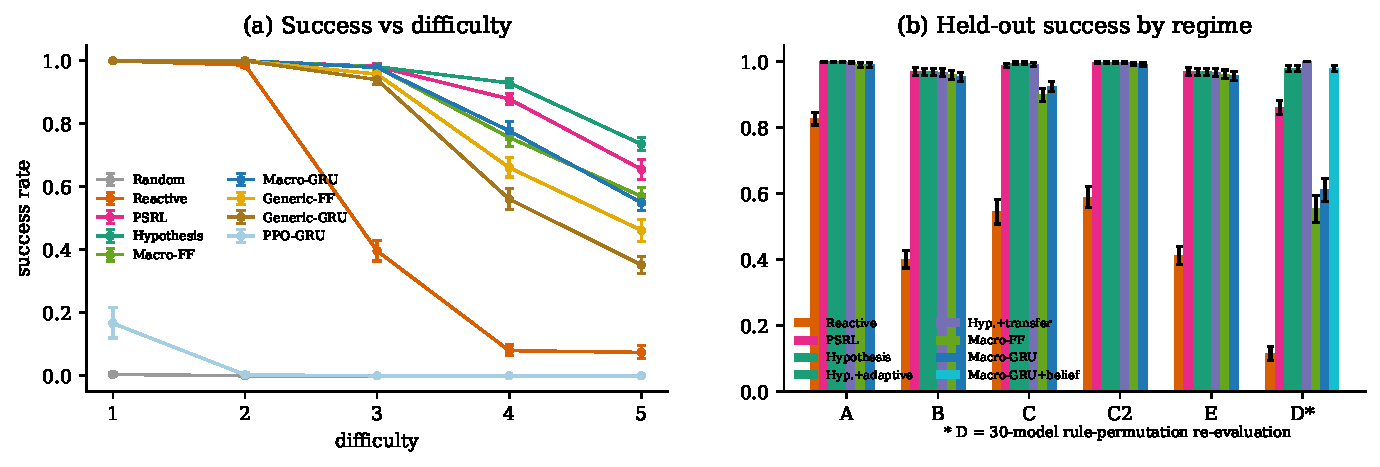
\includegraphics[width=\linewidth]{figures/fig15_main.pdf}
\caption{(a) Success versus difficulty; (b) held-out success per generalization regime (A--E, C2). Bars are 95\% bootstrap intervals over seeds.}\label{fig:main}
\end{figure}
\\subsection{Generalization to unseen compositions}
On the composition regimes (A, B, E; Table~\
ef{tab:gen}, Fig.~\
ef{fig:main}b) held-out success was 0.999, 0.969, 0.969 for the hypothesis agent, 0.827, 0.400, 0.412 reactive, 0.999, 0.971, 0.971 PSRL, 0.990, 0.953, 0.957 Macro-GRU. Growing the grid alone confounds size with difficulty, so structural generalization is split into longer dependency chains (C: 0.996 hypothesis, 0.544 reactive, 0.924 Macro-GRU) and size only (C2: gaps -0.024 and -0.208, i.e.\\ larger grids were not harder). The decisive contrast is the 30-seed rule-permutation re-evaluation on unseen colors. The hypothesis tracker scores 0.980, compared with 0.554 for Macro-FF, 0.611 for ordinary Macro-GRU, and 0.862 for PSRL. The matched-information Macro-GRU+belief also scores 0.980, while Hyp.+transfer reaches 1.000. The equality of Hypothesis and Macro-GRU+belief indicates that the large gap against ordinary learned policies is primarily due to structured access to uncertainty rather than the hypothesis-testing policy mechanism itself.

\\subsection{What matters: reward form, information bonus, memory and assumptions}
PSRL and the hypothesis agent differ in two ways: the reward is formed from a sampled binding or from expected value under confidences, and only the latter had an information bonus. A factorial design (Fig.~\
ef{fig:ablate}a; sampled-reward agents get the posterior-based bonus when $\\lambda>0$) shows at $d=5$ that the bonus ($\\lambda=8$ vs $0$) changed success from 0.682 to 0.873 for expected-value reward ($\\Delta=+0.191$, $p<0.001$) and from 0.657 to 0.791 for sampled reward ($\\Delta=+0.134$, $p<0.001$); holding $\\lambda$ fixed, expected-value reward versus sampled reward gave $\\Delta=+0.026$, $p=1.000$ at $\\lambda=0$ and $\\Delta=+0.082$, $p=0.003$ at $\\lambda=8$. Memory and revision are necessary: success was 0.928 with full memory and 0.000 with none, 0.928 with revision and 0.228 without; macro choice by expected value beat random macro choice (0.928 vs 0.814). Sweeping $\\lambda$ up to 8 (Fig.~\
ef{fig:lambda}), the bonus was significant at $d=4$ for $\\lambda=8$ and at $d=5$ for $\\lambda=1$, $\\lambda=2$, $\\lambda=4$, $\\lambda=8$, so it matters where distractors make uncertainty costly. Structural assumptions cut both ways (Fig.~\
ef{fig:ablate}b). The hypothesis agent assumes a key opens at most one door; when one key opens several doors it succeeded in 0.230 ($d=3$) and 0.182 ($d=4$) of episodes, versus 1.000 and 1.000 without the assumption, which in turn cost 0.120 when the assumption was true ($d=4$). PSRL, which resamples when its model offers no progress, was robust (1.000, 0.966).

\begin{figure}[t]
\centering
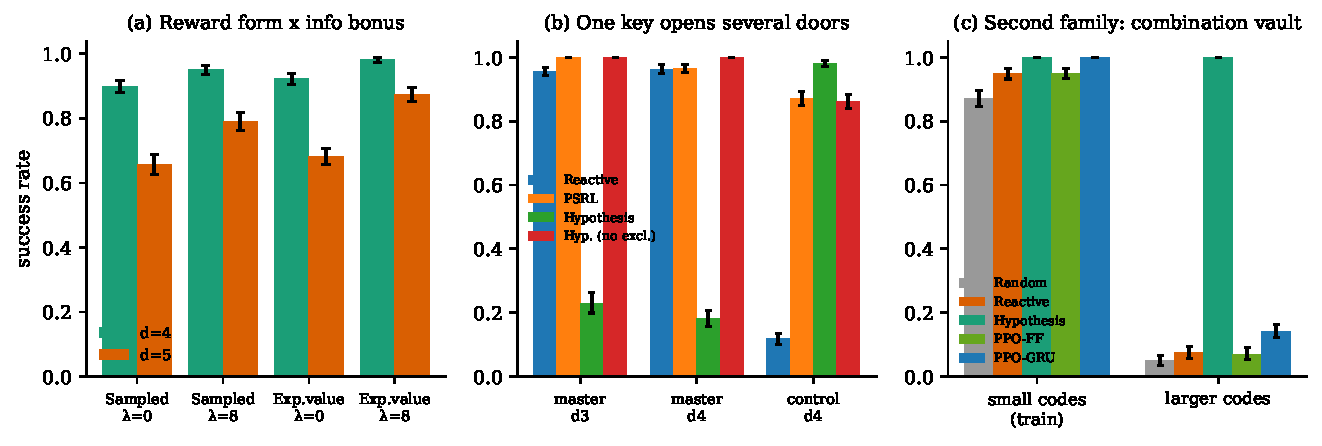
\includegraphics[width=\linewidth]{figures/fig16_ablate.pdf}
\caption{(a) Factorial ablation (difficulties 4 and 5); (b) master-key environments, where one key opens several doors, and an exclusive control; (c) the combination vault: small codes (training distribution) and larger codes.}\label{fig:ablate}
\end{figure}
\begin{figure}[t]
\centering
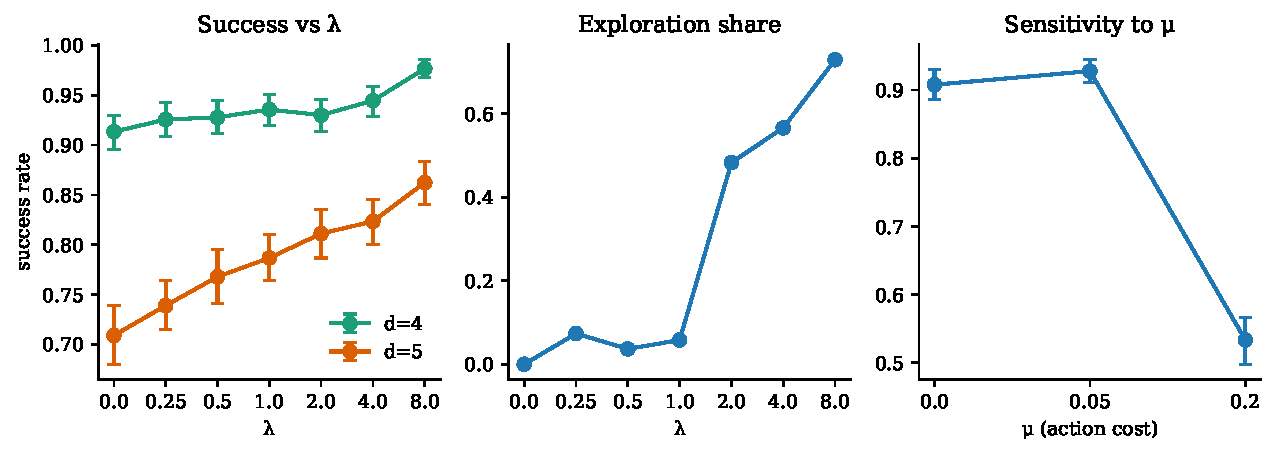
\includegraphics[width=.92\linewidth]{figures/fig10_explore_exploit.pdf}
\caption{Information-gain weight $\lambda$ (difficulties 4 and 5), exploration share, and action-cost weight $\mu$.}\label{fig:lambda}
\end{figure}
\egin{table}[t]
\\caption{Ablations at difficulty 4 (mean [95\\% CI]); $\\lambda$ weights the information bonus, $\\mu$ the action cost.}\\label{tab:abl}
\\centering\\setlength{\	abcolsep}{3pt}\\tiny
\egin{tabular}{lc}
\	oprule
Variant & Success \\\\
\\midrule
full\\_memory & 0.928 [0.911, 0.944] \\\\
no\\_memory & 0.000 [0.000, 0.000] \\\\
info\\_driven & 0.928 [0.911, 0.944] \\\\
random\\_explore & 0.814 [0.794, 0.834] \\\\
revision\\_on & 0.928 [0.911, 0.944] \\\\
revision\\_off & 0.228 [0.199, 0.256] \\\\
lambda\\_0.0 & 0.913 [0.896, 0.930] \\\\
lambda\\_0.5 & 0.928 [0.911, 0.944] \\\\
lambda\\_2.0 & 0.930 [0.913, 0.946] \\\\
lambda\\_8.0 & 0.977 [0.968, 0.986] \\\\
mu\\_0.0 & 0.908 [0.886, 0.930] \\\\
mu\\_0.2 & 0.533 [0.498, 0.567] \\\\
\ottomrule
\\end{tabular}
\\end{table}

\\subsection{Can the macro vocabulary be learned?}\\label{sec:vocab}
Generic-skill agents see only go-to-object skills and the primitives INTERACT and PUSH, so the testing structure (pick a key, try it on a door) must be discovered. At $d=3,4,5$ Generic-FF/GRU reached 0.958/0.940, 0.661/0.561 and 0.462/0.352, versus 0.980/0.979, 0.757/0.778 and 0.570/0.550 for Macro-FF/GRU. Macro-GRU was higher than Generic-GRU at $d=3$, $d=4$, $d=5$. Generic agents were trained for about 6k episodes (two seeds) against 12k for the macro agents; their training success had plateaued near 0.75, so a longer budget may close part of the gap, but we did not test this, and generic agents were not evaluated on the generalization regimes. The testing structure can therefore be learned from generic skills, at a cost that grows with difficulty.

\egin{table}[t]
\\caption{Spread across independently trained models of each learned agent (success rate).}\\label{tab:seeds}
\\centering\\setlength{\	abcolsep}{3pt}\\tiny
\egin{tabular}{lccccc}
\	oprule
Agent & Difficulty & Mean over training seeds & SD across training seeds & Min & Max \\\\
\\midrule
macro\\_ff & 3 & 0.98 & 0.009 & 0.97 & 0.987 \\\\
macro\\_ff & 4 & 0.757 & 0.018 & 0.737 & 0.77 \\\\
macro\\_ff & 5 & 0.57 & 0.033 & 0.533 & 0.597 \\\\
macro\\_gru & 3 & 0.979 & 0.008 & 0.97 & 0.987 \\\\
macro\\_gru & 4 & 0.778 & 0.005 & 0.773 & 0.783 \\\\
macro\\_gru & 5 & 0.55 & 0.006 & 0.547 & 0.557 \\\\
generic\\_ff & 3 & 0.958 & 0.006 & 0.953 & 0.962 \\\\
generic\\_ff & 4 & 0.661 & 0.02 & 0.647 & 0.676 \\\\
generic\\_ff & 5 & 0.462 & 0.006 & 0.458 & 0.467 \\\\
generic\\_gru & 3 & 0.94 & 0.016 & 0.929 & 0.951 \\\\
generic\\_gru & 4 & 0.561 & 0.011 & 0.553 & 0.569 \\\\
generic\\_gru & 5 & 0.352 & 0.036 & 0.327 & 0.378 \\\\
\ottomrule
\\end{tabular}
\\end{table}

\\subsection{A second family and the proposition}
In the combination vault (Fig.~\
ef{fig:ablate}c) the explicit hypothesis agent opened the vault in 1.000 of small-code and 1.000 of larger-code episodes, with 3.30 and 8.37 failed presses against the elimination predictions 3.33 and 8.32 of Proposition~1. On the grid, single-gate environments gave 0.271, 0.541, 0.779 failed door tests for $d=3,4,5$ against 0.287, 0.543, 0.801 predicted (computed with the number of keys reachable before the door opens), while the reactive agent made 0.289, 1.048, 1.541.  The learned vault agents mirror the grid findings: trained only on small codes, PPO-GRU reached 1.000 success (3.91 failed presses) in distribution but 0.142 on larger codes (84.0 failed presses), and PPO-FF 0.950 and 0.070, no better than the reactive agent (0.949, 0.074); learned memory solved the training distribution but did not extrapolate, whereas explicit elimination did.

\\subsection{Further checks}
\\emph{Rule types.} When some doors are opened by a switch rather than a key, the hypothesis agent with a closed vocabulary scored 0.469 and 0.254 and with an open vocabulary 1.000 and 0.999 ($d=3,4$); the reactive agent, which toggles every switch it sees, scored 0.962 and 0.951, so the agent chooses among rule types it was given rather than inventing them. \\emph{Recovery and priors.} After pre-training on identity-mapped rules, tests on mappings that violate them gave 0.780 with revision and 0.179 without, while an agent without the prior scored 1.000: cross-episode priors did not help when the relation persisted, and caused negative transfer when it was reversed. \\emph{Failures.} At $d=5$ the hypothesis agent failed 236 of 900 episodes; by fixed rules, distractor interference (189), long-horizon dependency (45), repeated refuted hypothesis (2). Raising the step budget from 200 to 800 lifts $d=5$ success from 0.74 to 0.87, so much of the residual is not a budget problem; we did not inspect causes episode by episode.
\begin{figure}[t]
\centering
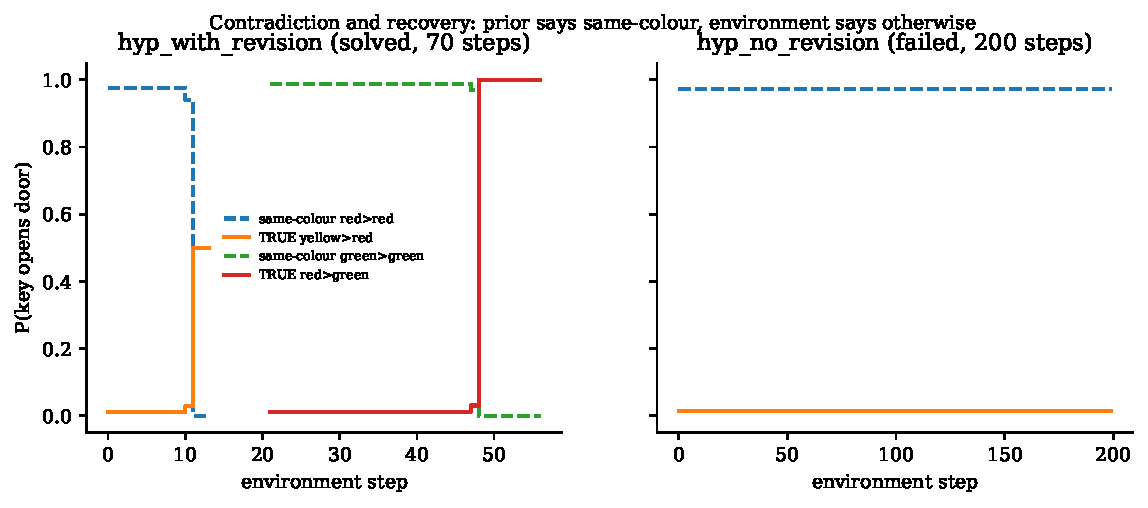
\includegraphics[width=.85\linewidth]{figures/fig8_contradiction_recovery.pdf}
\caption{Hypothesis probabilities in one held-out environment where a learned same-color prior is wrong: with revision the true bindings are found, without it the agent persists.}\label{fig:rec}
\end{figure}

\section{Discussion and Limitations}
\textbf{What drives performance.} Three layers separate. First, \emph{macro-action structure}: agents that choose among testable macro-actions substantially outperform reactive and primitive baselines. Second, \emph{structured evidence tracking}: memory, revision and information-seeking are important at the hardest levels. Third, \emph{representation of uncertainty versus policy mechanism}: at difficulty 5 the hypothesis tracker gains about 0.186 over ordinary Macro-GRU, while the matched-information Macro-GRU+belief removes essentially that gap. The 30-seed rule-permutation re-evaluation reproduces the pattern on unseen colors: Hypothesis 0.980, Macro-GRU+belief 0.980, Macro-GRU 0.611, Macro-FF 0.554, and PSRL 0.862. \textbf{Information versus learning.} Ordinary learned agents must infer both which uncertainty is relevant and how to act. The hypothesis tracker is given an explicit structured representation of uncertainty over candidate rules; Macro-GRU+belief receives the same representation but learns its policy. Their matched performance therefore attributes the large advantage over ordinary learned agents primarily to structured information access, not to hypothesis testing as a decision rule. \textbf{Costs of structure.} Assumptions that help when true are costly when false (master key), and cross-episode priors can hurt. \textbf{Limitations.} Both families are synthetic, deterministic and fully observable with hand-specified hypothesis spaces; macro-level agents receive a hand-built vocabulary, and generic skills are still hand-built. The learned baselines have finite training budgets, and primitive PPO is under-trained; constants were set by hand; steps-to-success is subject to survivor bias; we study no noise, language or foundation models, and nothing here supports claims of general intelligence.

\section{Conclusion}
In two structurally different benchmarks, agents that explicitly track evidence and test hypotheses reached near-optimal failed-test counts predicted by a simple elimination analysis. The matched-information comparison shows that the apparent advantage over ordinary learned policies is largely explained by structured access to uncertainty over hidden rules: a learned Macro-GRU supplied with the tracker's beliefs matches the hypothesis tracker at the hardest difficulty. The 30-seed rule-permutation evaluation reproduces this result on unseen color symbols, with Hypothesis 0.980 and Macro-GRU+belief 0.980, while ordinary Macro-GRU reaches 0.611 and PSRL 0.862. Thus the central distinction in this benchmark is not hypothesis-based versus learned decision making, but structured belief access versus implicit inference of the relevant uncertainty state. Future work should test whether the structured uncertainty representation itself can be learned from lower-level observations and whether the same decomposition survives under stochastic, noisy and less hand-structured environments.

\section{Reproducibility}
Code, tests, configuration and the one-command pipeline are in the supplementary archive; every number is read from \texttt{data/results/*.csv} by \texttt{paper/build\_paper.py}, and secondary tables (ablations, scaling, all significance tests) are in \texttt{paper/tables/}. Everything runs on one CPU core with 3~GB RAM. We found and fixed several bugs in our own agents and baselines before reporting (refuted-hypothesis retest loops, a posterior-sampling sample that assigned an unreachable key, two defects in the shaping signal of primitive PPO, and an evaluation stage that overwrote results); no pre-fix results appear here.

\bibliographystyle{splncs04}
\bibliography{references}
\end{document}
